\section{Ergebnisse}
%xy anpassen!!!
Die in Abschnitt 3.2 beschriebene Netzstruktur wird mit dem in Abschnitt 3.3 vorgestelltem Datensatz und Parametern trainiert und validiert. Die optimalen Trainingsparameter wurden dabei aus mehren Experimenten empirisch ermittelt. Dabei dient die in Abschnitt 3.1 erarbeitete \textit{Loss}-Metrik zur jeweiligen Quantisierung des Trainingserfolges. \\Abbildung \ref{lossbild} zeigt den Verlauf des \textit{Loss} über die Trainingsiterationen im 3D-Fall. Die Variable \textit{loss} steht für den \textit{Loss}  der Trainingsdaten und \textit{val\_loss} für den \textit{Loss} der Testdaten. Dabei fällt dieser zunächst relativ schnell und nähert sich dann XY an. Dies deutet auf ein erfolgreiches Training ohne \textit{Overfitting} hin. 
 
\begin{figure}[!htb] 
  \centering
  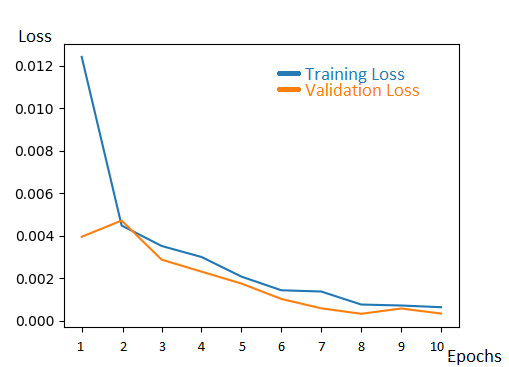
\includegraphics[width=13.8cm]{Abb/training_progress.png}
  \caption{Loss und Val über Trainingsepochen}
  \label{lossbild}
\end{figure} 
In Abbildung 11 und 12 werden beispielhaft zwei prädizierte Bounding-Boxen der Testdaten dargestellt (blau). Zum Vergleich sind zusätzlich die manuell vorgelabelten Bounding-Boxen eingezeichnet (rot). Oben im Bild steht der jeweils errechnete \textit{Loss}. Hier ist zu erkennen, dass das rechte Bild mit dem höchsten \textit{Loss} auch die sichtbar größte Abweichung der prädizierten Bounding-Box mit der vorgelabelten aufweist. Der \textit{Loss} im linken Bild ist relativ gering und spiegelt so auch die erkennbare Ähnlichkeit der prädizierten Bounding-Box zur vorgelabelten Bounding-Box wieder.\\ \label{pred_boxes}
\begin{figure}[!htb]
   \begin{minipage}[b]{.5\linewidth} % [b] => Ausrichtung an \caption
      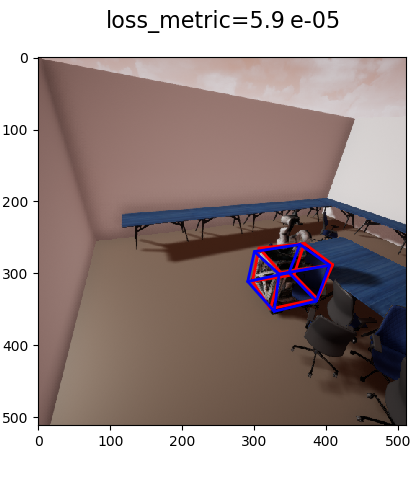
\includegraphics[width=\linewidth]{bbs/gut.png}  
      \label{tiv_ausgang}    
      \caption{Beispiel einer gut prädizierten Bounding-Box mit geringem Loss. Zu sehen ist die gelabelte Bounding-Box (rot), sowie die prädizierte Bounding-Box (blau)}
   \end{minipage}
   \hspace{.03\linewidth}% Abstand zwischen Bilder
   \begin{minipage}[b]{.5\linewidth} % [b] => Ausrichtung an \caption
      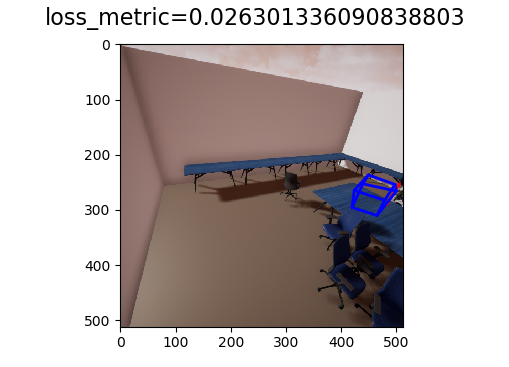
\includegraphics[width=\linewidth]{bbs/schlecht.png}
      \label{vdiffX_unsymm} 
      \caption{Beispiel einer schlecht prädizierten Bounding-Box mit hohem Loss. Hier könnte speziell der Stuhl und der Tisch das Netzwerk beeinflusst haben}
   \end{minipage}
\end{figure}
\newpage